\documentclass[11pt,a4paper]{report}
%\usepackage[utf8]{inputenc}
\usepackage[latin1]{inputenc}
\usepackage{amsmath}
\usepackage{amsfonts}
\usepackage{amssymb}
\usepackage{multicol, blindtext}
\usepackage[top=0.58in, bottom=0.9in]{geometry}
\usepackage{textcomp}
\usepackage{graphicx}
\usepackage{lipsum}

\title{	\begin{figure}[h]
			\centering
			
\includegraphics[scale=0.75]{./pictures/logoufpa.png}
			\label{fig:logoufpa}
		\end{figure}
		Universidade Federal do Par� \linebreak
		Instituto de Tecnologia \linebreak
		Faculdade de Engenharia de Computa��o e Telecomunica��es \linebreak
		Sistemas de Controle \linebreak
		Experi�ncia 4 (Projeto por aloca��o de p�los) com $MatLab^{\copyright}$ \linebreak
		Prof$^{a}$ Adriana Castro}

\begin{document}

\author{Danilo Souza - 10080000801}
\maketitle

\tableofcontents
\listoffigures

\chapter{Experimento 1}

	As Figuras \ref{fig:experimento1_LGR_original}, \ref{fig:experimento1_LGR_zero} e \ref{fig:experimento1_LGR_polo} mostram, respectivamente, o LGR de $G(s) = \frac{2}{s(s+1)}$, o LGR de $G(s) = \frac{2(s+2)}{s(s+1)}$e o LGR de $G(s) = \frac{2}{s(s+1)(s+2)}$. Quando um zero � adiconado ao LGR, o sistema permanece est�vel para qualquer valor positivo de $K$ ($K \geqslant 0$). Quando um p�lo � adicionado ao LRG, conforme o servado abaixo, o LGR entra para o plano da instalbilidade (SPD), fazendo com que o valor de K possua uma faixa limitada de estabilidade que neste caso � $K \leqslant 3$.
	
		\begin{figure}[h!]
			\centering
			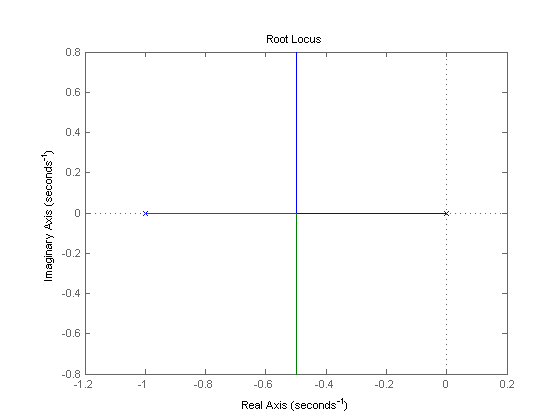
\includegraphics[scale=0.6]{./pictures/experimento1_LGR_original.png}
			\caption{LGR origial do experimento 1}
			\label{fig:experimento1_LGR_original}
		\end{figure}
		\begin{figure}[h!]
			\centering
			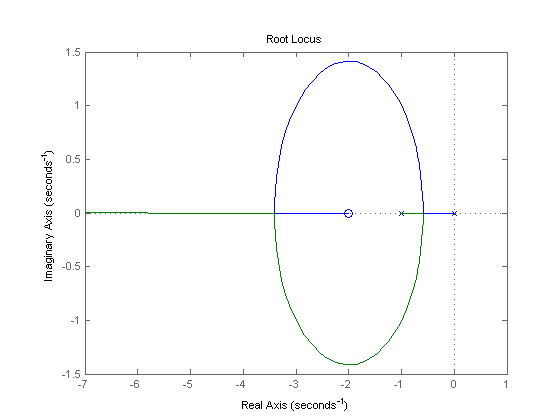
\includegraphics[scale=0.6]{./pictures/experimento1_LGR_zero.png}
			\caption{LGR com adi��o de umz zero do experimento 1}
			\label{fig:experimento1_LGR_zero}
		\end{figure}
		\begin{figure}[h!]
			\centering
			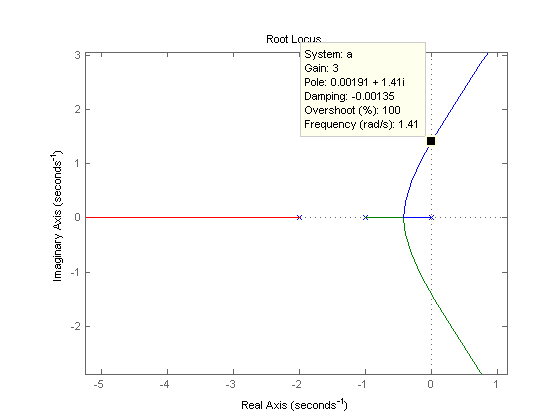
\includegraphics[scale=0.6]{./pictures/experimento1_LGR_polo.png}
			\caption{LGR com adi��o de um p�lo do experimento 1}
			\label{fig:experimento1_LGR_polo}
		\end{figure}
	

\chapter{Experimento 2}

\chapter{Experimento 3}

	Usando a tabela fornecida podemos encontra o valor de $R$ para $T_{s} = 3$. A Figura \ref{fig:experimento3_ganho} mostra o valor do ganho para o valor de $R$ encontrado. 
		\[ T_{s_{5\%}}  = -\frac{3}{R} \rightarrow R = -1 \]
	A Figura \ref{fig:experimento3_resposta} mostra a resposta do sistema simulado em malha fechada, o valor encontrado foi $T_{s} = 3,024$, confirmando o tempo de resposta desejado $T_{s_{desejado}} = 3$ .
		
		\begin{figure}[h!]
			\centering
			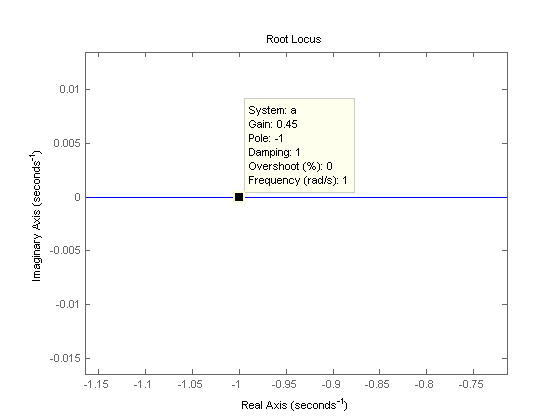
\includegraphics[scale=0.6]{./pictures/experimento3_ganho.png}
			\caption{Ganho do experimento 3}
			\label{fig:experimento3_ganho}
		\end{figure}
		\begin{figure}[h!]
			\centering
			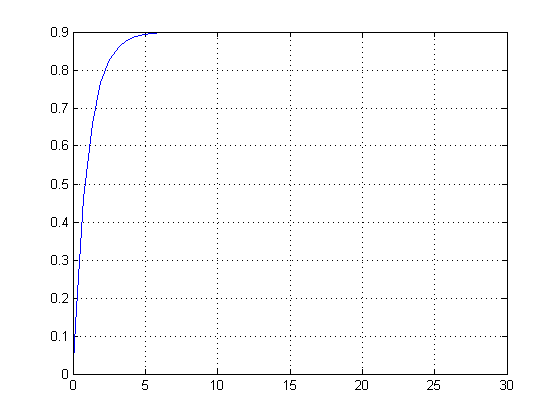
\includegraphics[scale=0.6]{./pictures/experimento3_resposta.png}
			\caption{Resposta do sistema simulado em malha fechada}
			\label{fig:experimento3_resposta}
		\end{figure}	

\chapter{Experimento 4}

	A Figura \ref{fig:experimento4_LGR} mostra o LGR e o ganho para que o sistema $G(s) = \frac{2}{s(s+1)}$ tenha sobre-sinal de 5\% ($M_{p} = 0,05$). A Figura \ref{fig:experimento4_resposta} mostra a resposta do sistema em malha fechada, o valor de encontrado foi $M_{p} = 0,49$ confirmando o valor desejado.
	
		\begin{figure}[h!]
			\centering
			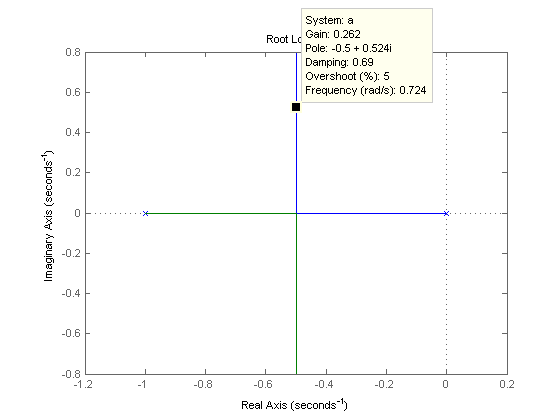
\includegraphics[scale=0.6]{./pictures/experimento4_LGR.png}
			\caption{LGR e ganho do experimento 4}
			\label{fig:experimento4_LGR}
		\end{figure}
		\begin{figure}[h!]
			\centering
			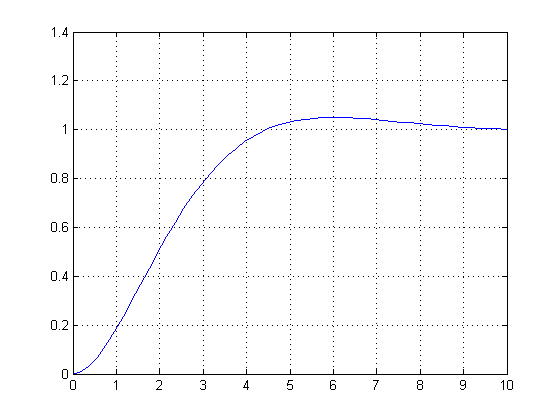
\includegraphics[scale=0.6]{./pictures/experimento4_resposta.png}
			\caption{Resposta do sistema simulado em malha fechada}
			\label{fig:experimento4_resposta}
		\end{figure}	
		
\end{document}
